%! TEX root = ../main.tex
% =============================================================
% IMMUTABLE — generated automatically, do not edit this block
%   script          : analysis_scratch/mansard_funke.py
%   plot_type       : mansard_funke_reflection
%   chapter         : 04
%   probes          : 8804/250, 9373/170
%   delta_mm        : 569
%   n_primary_nowind: 50
% =============================================================
\begin{figure}[htbp]
  \centering
  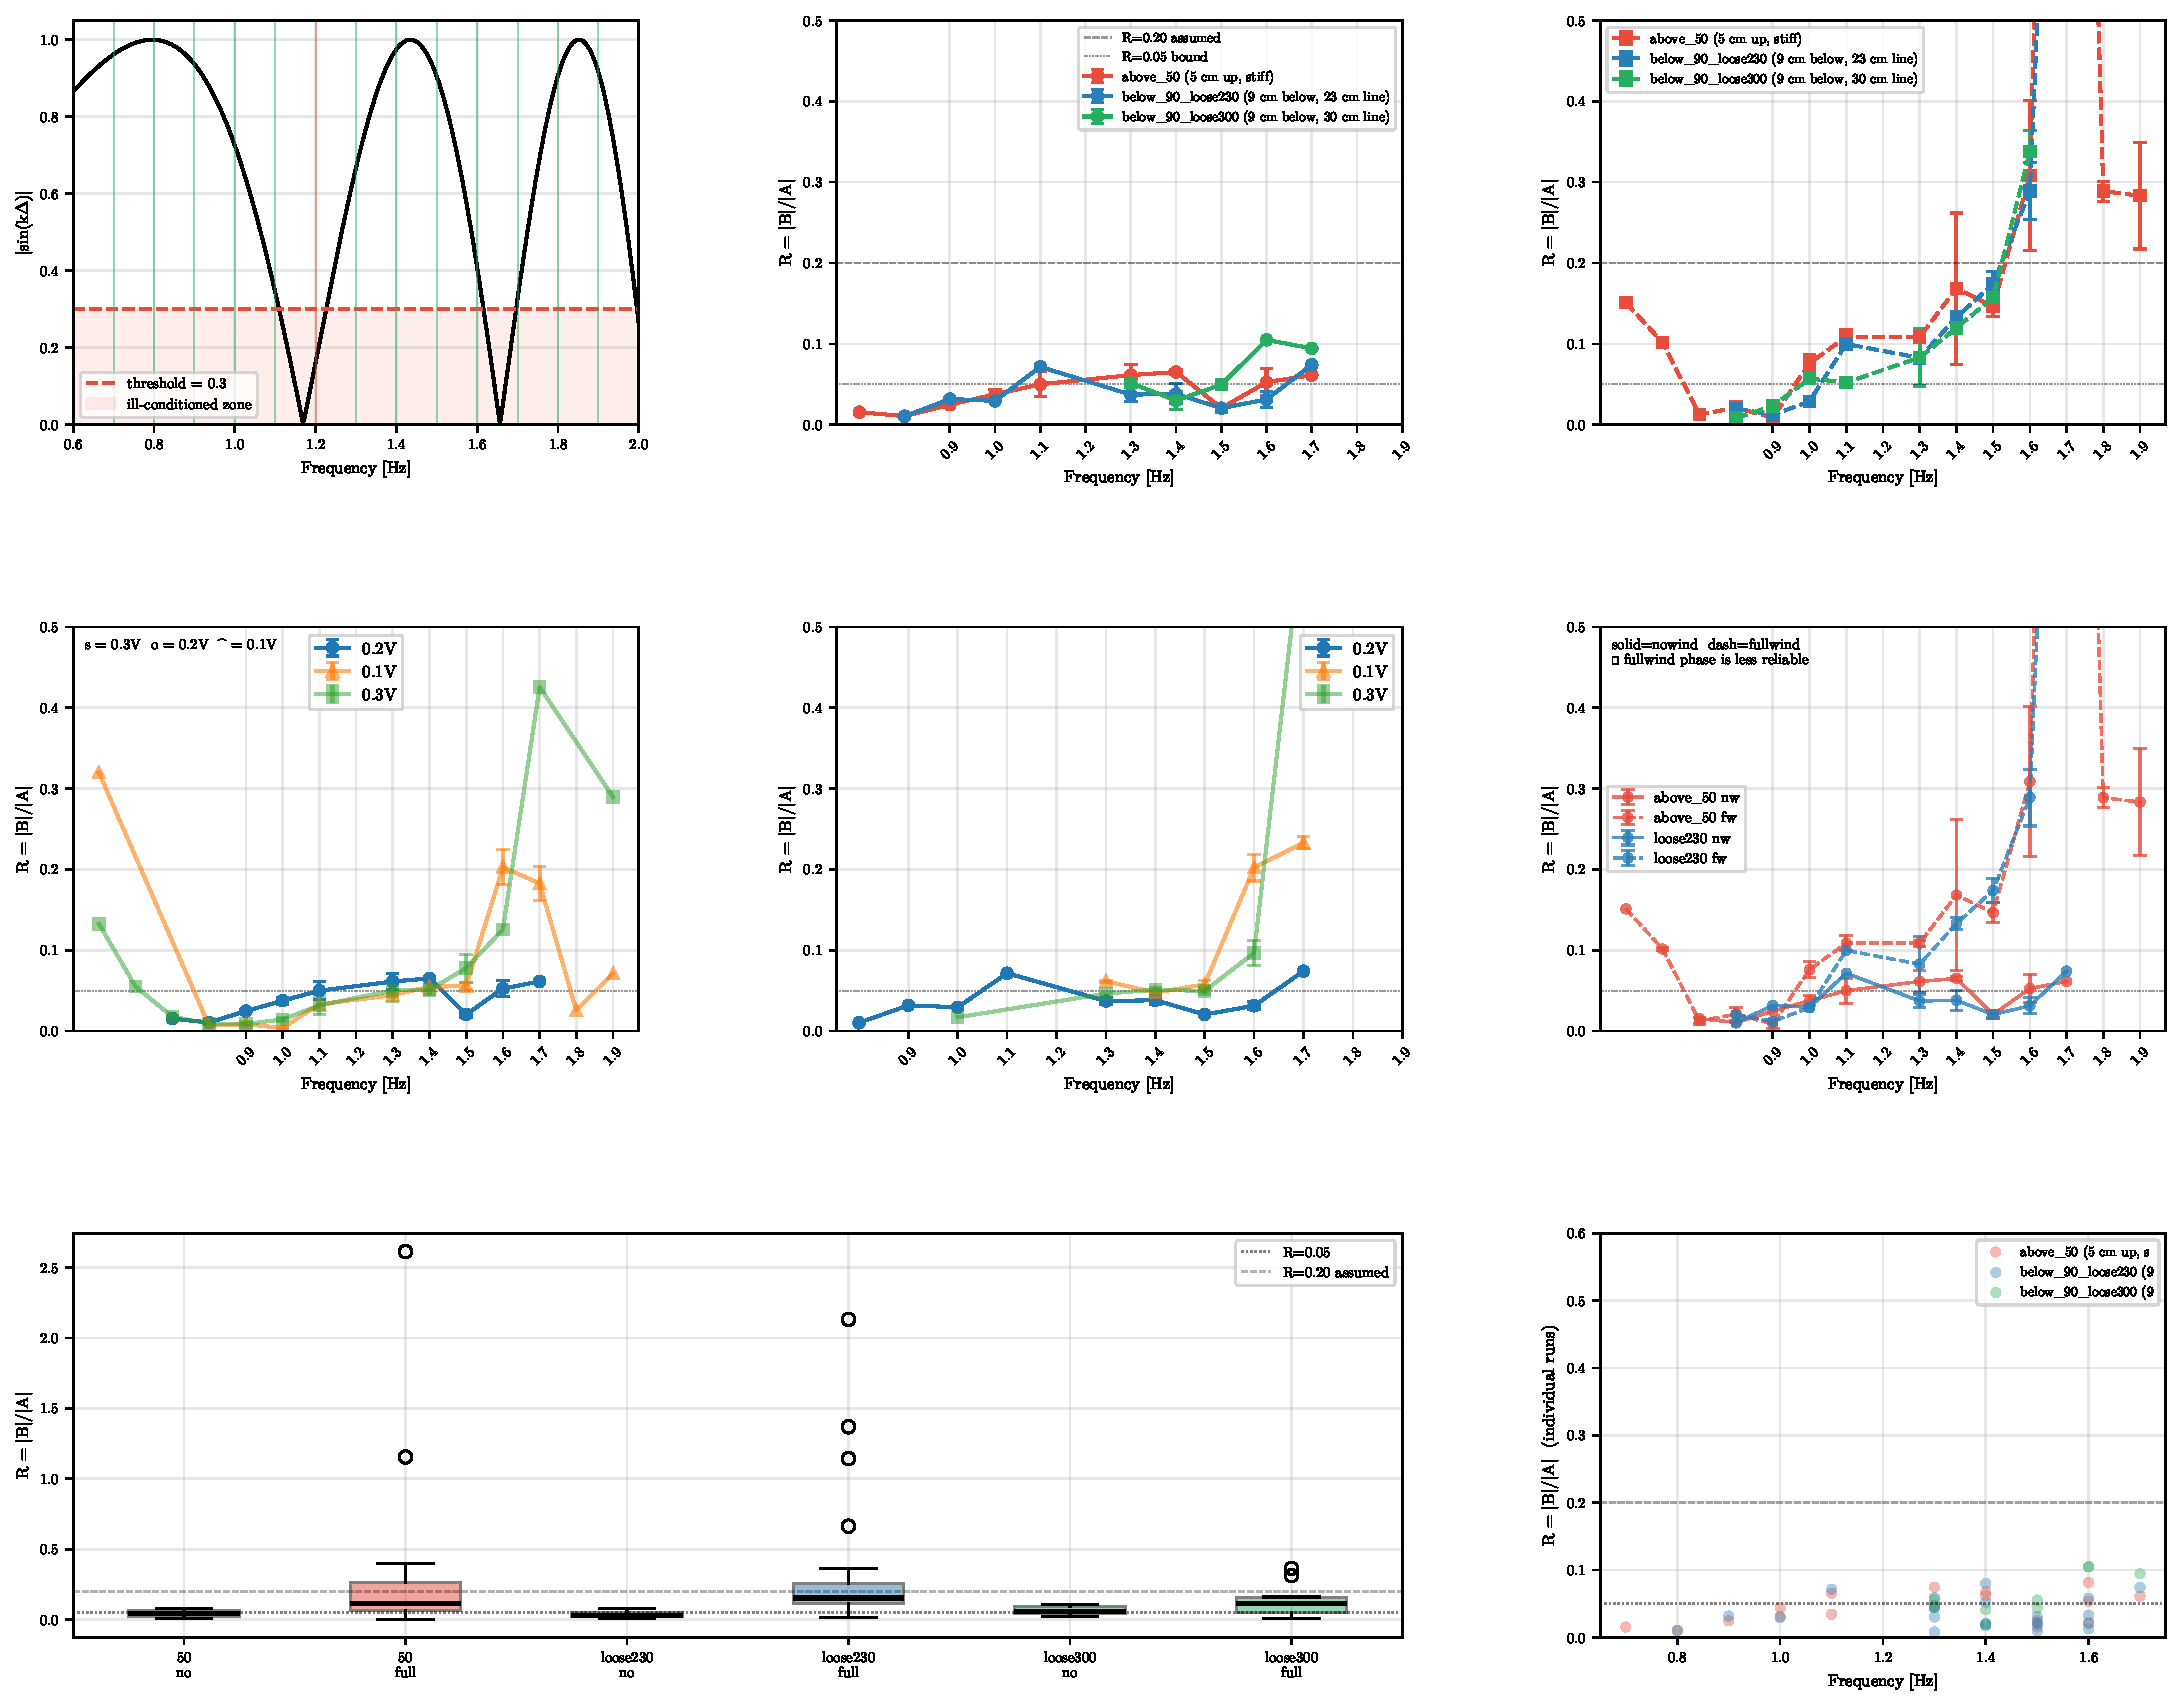
\includegraphics[width=0.95\linewidth]{FIGURES/ch04_mansard_funke_reflection.pdf}
  \caption[Mansard--Funke reflection analysis]{%
    Mansard--Funke two-probe reflection analysis using 8804/250 (upstream) and 9373/170 (IN probe), $\Delta x = 569$\,mm. Panels: (A) MF conditioning $|\sin(k\Delta x)|$ vs frequency (dashed: ill-conditioned threshold 0.30); (B) R vs freq, nowind 0.2\,V, by mooring; (C) R vs freq, fullwind 0.2\,V, by mooring; (D) R histogram all moorings; (E--G) amplitude-tier diagnostics; (H) R distribution box-plot by mooring and wind; (I) run-level R scatter. Result: at 0.2\,V nowind, median R per mooring = above_50 0.047, b90_loose230 0.049, b90_loose300 0.048 (n=50). R$\ll$0.20 supports the decision to apply no standing-wave correction to OUT/IN (FFT).
  }
  \label{fig:ch04_mansard_funke_reflection}
\end{figure}
